% ImageNet 64x64 训练曲线 — CC-iGPT v1 (12ep cosine, in-training)
% 编译: pdflatex imagenet64_training_curves.tex   (或 latexmk -pdf)
% 嵌入论文: % ImageNet 64x64 训练曲线 — CC-iGPT v1 (12ep cosine, in-training)
% 编译: pdflatex imagenet64_training_curves.tex   (或 latexmk -pdf)
% 嵌入论文: % ImageNet 64x64 训练曲线 — CC-iGPT v1 (12ep cosine, in-training)
% 编译: pdflatex imagenet64_training_curves.tex   (或 latexmk -pdf)
% 嵌入论文: % ImageNet 64x64 训练曲线 — CC-iGPT v1 (12ep cosine, in-training)
% 编译: pdflatex imagenet64_training_curves.tex   (或 latexmk -pdf)
% 嵌入论文: \input{figures/imagenet64_training_curves.tex}
%
% 数据来源: experiments/ccigpt_imagenet64_v1_train.log（截至 ep9/12 完成，2026-06-05）
%   ep | train_bpd | val_bpd | LR
%    1 |   4.3969  |  3.6624 | 3.00e-04
%    2 |   3.5751  |  3.5834 | 3.00e-04
%    3 |   3.5127  |  3.5523 | 2.94e-04
%    4 |   3.4825  |  3.5358 | 2.77e-04
%    5 |   3.4654  |  3.5217 | 2.51e-04
%    6 |   3.4545  |  3.5147 | 2.17e-04
%    7 |   3.4429  |  3.5048 | 1.78e-04
%    8 |   3.4368  |  3.4994 | 1.37e-04
%    9 |   3.4268  |  3.4931 | 9.83e-05
%
% ！进行中：ep10-12 待回填（ep9 已完成）。val 已低于 SPN 3.52，距目标 3.44 剩 0.0531；
%   cosine 退火尾段在走（ep5→9 LR 2.51→0.983e-4），最终 3.44 判定待 ep12（ETA 06-08~10）。
\documentclass[tikz,border=8pt]{standalone}
\usepackage{tikz}
\usepackage{pgfplots}
\usepackage{amsmath,amssymb}
\pgfplotsset{compat=1.18}

\begin{document}
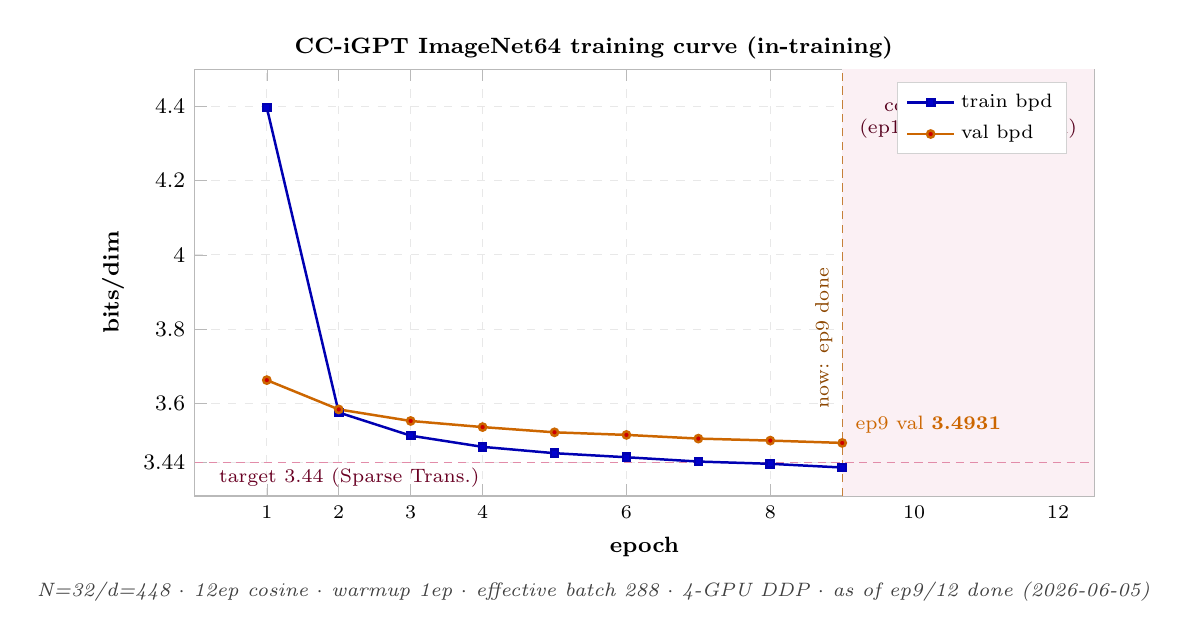
\begin{tikzpicture}[font=\footnotesize]
\begin{axis}[
    width=13cm, height=7cm,
    xlabel={\textbf{epoch}},
    ylabel={\textbf{bits/dim}},
    ylabel near ticks,
    xlabel near ticks,
    xmin=0, xmax=12.5,
    ymin=3.35, ymax=4.5,
    ytick={3.44,3.6,3.8,4.0,4.2,4.4},
    xtick={1,2,3,4,6,8,10,12},
    x tick label style={font=\scriptsize},
    axis line style={gray!55},
    tick style={gray!55},
    grid=major,
    grid style={dashed, gray!18, line width=0.3pt},
    legend style={
        font=\scriptsize,
        draw=gray!35, fill=white,
        at={(0.97,0.97)}, anchor=north east,
        cells={anchor=west},
        row sep=1pt,
    },
    clip=false,
]

% --- 退火尾段区间底纹 (ep10-12，待回填) ---
\fill[purple!6] (axis cs:9,3.35) rectangle (axis cs:12.5,4.5);
\node[font=\scriptsize, purple!45!black, anchor=north, align=center]
    at (axis cs:10.75, 4.45) {cosine anneal tail\\(ep10--12, not yet run)};

% --- 当前进度竖虚线 (ep9 done) ---
\draw[densely dashed, gray!45!orange, line width=0.4pt]
    (axis cs:9, 3.35) -- (axis cs:9, 4.5);
\node[font=\scriptsize, orange!55!black, anchor=south west, rotate=90]
    at (axis cs:9, 3.55) {\,now: ep9 done};

% --- 目标线 3.44 (Sparse Transformer) ---
\draw[densely dashed, purple!45, line width=0.5pt]
    (axis cs:0,3.44) -- (axis cs:12.5,3.44);
\node[font=\scriptsize, purple!55!black, anchor=west]
    at (axis cs:0.2, 3.40) {target 3.44 (Sparse Trans.)};

% --- train_bpd 曲线 (9 点) ---
\addplot+[
    mark=square*, mark size=1.3pt, line width=0.9pt, color=blue!70!black,
] coordinates {
    (1, 4.3969)
    (2, 3.5751)
    (3, 3.5127)
    (4, 3.4825)
    (5, 3.4654)
    (6, 3.4545)
    (7, 3.4429)
    (8, 3.4368)
    (9, 3.4268)
};
\addlegendentry{train bpd}

% --- val_bpd 曲线 (9 点) ---
\addplot+[
    mark=*, mark size=1.3pt, line width=0.9pt, color=orange!80!black,
] coordinates {
    (1, 3.6624)
    (2, 3.5834)
    (3, 3.5523)
    (4, 3.5358)
    (5, 3.5217)
    (6, 3.5147)
    (7, 3.5048)
    (8, 3.4994)
    (9, 3.4931)
};
\addlegendentry{val bpd}

% --- ep9 末点标注 ---
\node[font=\scriptsize, orange!80!black, anchor=south west]
    at (axis cs:9.05, 3.4931) {ep9 val \textbf{3.4931}};

\end{axis}

% --- 标题 ---
\node[font=\footnotesize\bfseries, anchor=south]
    at (current bounding box.north)
    {CC-iGPT ImageNet64 training curve (in-training)};

% --- 副标题（配置） ---
\node[font=\scriptsize, gray!50!black, anchor=north, yshift=-2pt]
    at (current bounding box.south)
    {\textit{N=32/d=448 $\cdot$ 12ep cosine $\cdot$ warmup 1ep $\cdot$ effective batch 288 $\cdot$ 4-GPU DDP $\cdot$ as of ep9/12 done (2026-06-05)}};

\end{tikzpicture}
\end{document}

%
% 数据来源: experiments/ccigpt_imagenet64_v1_train.log（截至 ep9/12 完成，2026-06-05）
%   ep | train_bpd | val_bpd | LR
%    1 |   4.3969  |  3.6624 | 3.00e-04
%    2 |   3.5751  |  3.5834 | 3.00e-04
%    3 |   3.5127  |  3.5523 | 2.94e-04
%    4 |   3.4825  |  3.5358 | 2.77e-04
%    5 |   3.4654  |  3.5217 | 2.51e-04
%    6 |   3.4545  |  3.5147 | 2.17e-04
%    7 |   3.4429  |  3.5048 | 1.78e-04
%    8 |   3.4368  |  3.4994 | 1.37e-04
%    9 |   3.4268  |  3.4931 | 9.83e-05
%
% ！进行中：ep10-12 待回填（ep9 已完成）。val 已低于 SPN 3.52，距目标 3.44 剩 0.0531；
%   cosine 退火尾段在走（ep5→9 LR 2.51→0.983e-4），最终 3.44 判定待 ep12（ETA 06-08~10）。
\documentclass[tikz,border=8pt]{standalone}
\usepackage{tikz}
\usepackage{pgfplots}
\usepackage{amsmath,amssymb}
\pgfplotsset{compat=1.18}

\begin{document}
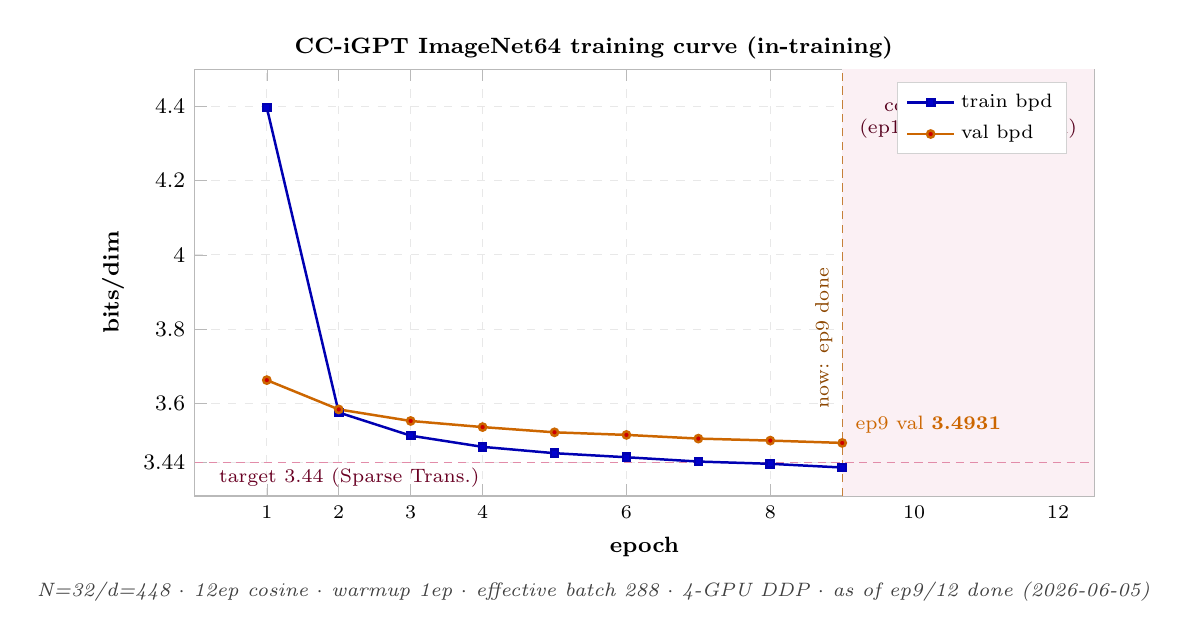
\begin{tikzpicture}[font=\footnotesize]
\begin{axis}[
    width=13cm, height=7cm,
    xlabel={\textbf{epoch}},
    ylabel={\textbf{bits/dim}},
    ylabel near ticks,
    xlabel near ticks,
    xmin=0, xmax=12.5,
    ymin=3.35, ymax=4.5,
    ytick={3.44,3.6,3.8,4.0,4.2,4.4},
    xtick={1,2,3,4,6,8,10,12},
    x tick label style={font=\scriptsize},
    axis line style={gray!55},
    tick style={gray!55},
    grid=major,
    grid style={dashed, gray!18, line width=0.3pt},
    legend style={
        font=\scriptsize,
        draw=gray!35, fill=white,
        at={(0.97,0.97)}, anchor=north east,
        cells={anchor=west},
        row sep=1pt,
    },
    clip=false,
]

% --- 退火尾段区间底纹 (ep10-12，待回填) ---
\fill[purple!6] (axis cs:9,3.35) rectangle (axis cs:12.5,4.5);
\node[font=\scriptsize, purple!45!black, anchor=north, align=center]
    at (axis cs:10.75, 4.45) {cosine anneal tail\\(ep10--12, not yet run)};

% --- 当前进度竖虚线 (ep9 done) ---
\draw[densely dashed, gray!45!orange, line width=0.4pt]
    (axis cs:9, 3.35) -- (axis cs:9, 4.5);
\node[font=\scriptsize, orange!55!black, anchor=south west, rotate=90]
    at (axis cs:9, 3.55) {\,now: ep9 done};

% --- 目标线 3.44 (Sparse Transformer) ---
\draw[densely dashed, purple!45, line width=0.5pt]
    (axis cs:0,3.44) -- (axis cs:12.5,3.44);
\node[font=\scriptsize, purple!55!black, anchor=west]
    at (axis cs:0.2, 3.40) {target 3.44 (Sparse Trans.)};

% --- train_bpd 曲线 (9 点) ---
\addplot+[
    mark=square*, mark size=1.3pt, line width=0.9pt, color=blue!70!black,
] coordinates {
    (1, 4.3969)
    (2, 3.5751)
    (3, 3.5127)
    (4, 3.4825)
    (5, 3.4654)
    (6, 3.4545)
    (7, 3.4429)
    (8, 3.4368)
    (9, 3.4268)
};
\addlegendentry{train bpd}

% --- val_bpd 曲线 (9 点) ---
\addplot+[
    mark=*, mark size=1.3pt, line width=0.9pt, color=orange!80!black,
] coordinates {
    (1, 3.6624)
    (2, 3.5834)
    (3, 3.5523)
    (4, 3.5358)
    (5, 3.5217)
    (6, 3.5147)
    (7, 3.5048)
    (8, 3.4994)
    (9, 3.4931)
};
\addlegendentry{val bpd}

% --- ep9 末点标注 ---
\node[font=\scriptsize, orange!80!black, anchor=south west]
    at (axis cs:9.05, 3.4931) {ep9 val \textbf{3.4931}};

\end{axis}

% --- 标题 ---
\node[font=\footnotesize\bfseries, anchor=south]
    at (current bounding box.north)
    {CC-iGPT ImageNet64 training curve (in-training)};

% --- 副标题（配置） ---
\node[font=\scriptsize, gray!50!black, anchor=north, yshift=-2pt]
    at (current bounding box.south)
    {\textit{N=32/d=448 $\cdot$ 12ep cosine $\cdot$ warmup 1ep $\cdot$ effective batch 288 $\cdot$ 4-GPU DDP $\cdot$ as of ep9/12 done (2026-06-05)}};

\end{tikzpicture}
\end{document}

%
% 数据来源: experiments/ccigpt_imagenet64_v1_train.log（截至 ep9/12 完成，2026-06-05）
%   ep | train_bpd | val_bpd | LR
%    1 |   4.3969  |  3.6624 | 3.00e-04
%    2 |   3.5751  |  3.5834 | 3.00e-04
%    3 |   3.5127  |  3.5523 | 2.94e-04
%    4 |   3.4825  |  3.5358 | 2.77e-04
%    5 |   3.4654  |  3.5217 | 2.51e-04
%    6 |   3.4545  |  3.5147 | 2.17e-04
%    7 |   3.4429  |  3.5048 | 1.78e-04
%    8 |   3.4368  |  3.4994 | 1.37e-04
%    9 |   3.4268  |  3.4931 | 9.83e-05
%
% ！进行中：ep10-12 待回填（ep9 已完成）。val 已低于 SPN 3.52，距目标 3.44 剩 0.0531；
%   cosine 退火尾段在走（ep5→9 LR 2.51→0.983e-4），最终 3.44 判定待 ep12（ETA 06-08~10）。
\documentclass[tikz,border=8pt]{standalone}
\usepackage{tikz}
\usepackage{pgfplots}
\usepackage{amsmath,amssymb}
\pgfplotsset{compat=1.18}

\begin{document}
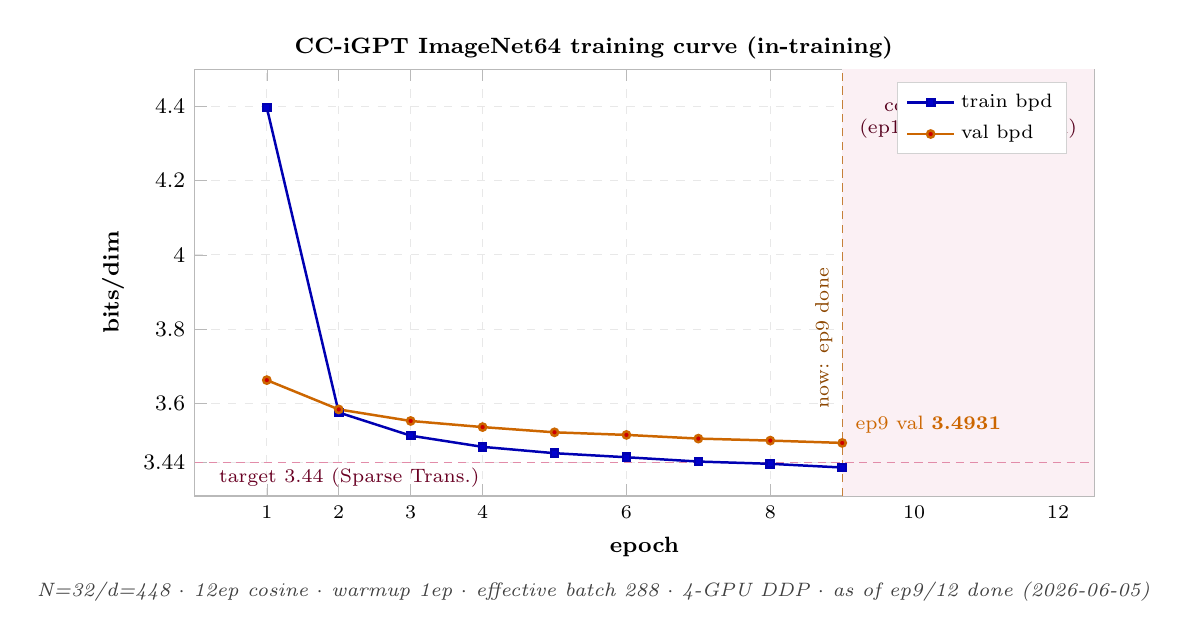
\begin{tikzpicture}[font=\footnotesize]
\begin{axis}[
    width=13cm, height=7cm,
    xlabel={\textbf{epoch}},
    ylabel={\textbf{bits/dim}},
    ylabel near ticks,
    xlabel near ticks,
    xmin=0, xmax=12.5,
    ymin=3.35, ymax=4.5,
    ytick={3.44,3.6,3.8,4.0,4.2,4.4},
    xtick={1,2,3,4,6,8,10,12},
    x tick label style={font=\scriptsize},
    axis line style={gray!55},
    tick style={gray!55},
    grid=major,
    grid style={dashed, gray!18, line width=0.3pt},
    legend style={
        font=\scriptsize,
        draw=gray!35, fill=white,
        at={(0.97,0.97)}, anchor=north east,
        cells={anchor=west},
        row sep=1pt,
    },
    clip=false,
]

% --- 退火尾段区间底纹 (ep10-12，待回填) ---
\fill[purple!6] (axis cs:9,3.35) rectangle (axis cs:12.5,4.5);
\node[font=\scriptsize, purple!45!black, anchor=north, align=center]
    at (axis cs:10.75, 4.45) {cosine anneal tail\\(ep10--12, not yet run)};

% --- 当前进度竖虚线 (ep9 done) ---
\draw[densely dashed, gray!45!orange, line width=0.4pt]
    (axis cs:9, 3.35) -- (axis cs:9, 4.5);
\node[font=\scriptsize, orange!55!black, anchor=south west, rotate=90]
    at (axis cs:9, 3.55) {\,now: ep9 done};

% --- 目标线 3.44 (Sparse Transformer) ---
\draw[densely dashed, purple!45, line width=0.5pt]
    (axis cs:0,3.44) -- (axis cs:12.5,3.44);
\node[font=\scriptsize, purple!55!black, anchor=west]
    at (axis cs:0.2, 3.40) {target 3.44 (Sparse Trans.)};

% --- train_bpd 曲线 (9 点) ---
\addplot+[
    mark=square*, mark size=1.3pt, line width=0.9pt, color=blue!70!black,
] coordinates {
    (1, 4.3969)
    (2, 3.5751)
    (3, 3.5127)
    (4, 3.4825)
    (5, 3.4654)
    (6, 3.4545)
    (7, 3.4429)
    (8, 3.4368)
    (9, 3.4268)
};
\addlegendentry{train bpd}

% --- val_bpd 曲线 (9 点) ---
\addplot+[
    mark=*, mark size=1.3pt, line width=0.9pt, color=orange!80!black,
] coordinates {
    (1, 3.6624)
    (2, 3.5834)
    (3, 3.5523)
    (4, 3.5358)
    (5, 3.5217)
    (6, 3.5147)
    (7, 3.5048)
    (8, 3.4994)
    (9, 3.4931)
};
\addlegendentry{val bpd}

% --- ep9 末点标注 ---
\node[font=\scriptsize, orange!80!black, anchor=south west]
    at (axis cs:9.05, 3.4931) {ep9 val \textbf{3.4931}};

\end{axis}

% --- 标题 ---
\node[font=\footnotesize\bfseries, anchor=south]
    at (current bounding box.north)
    {CC-iGPT ImageNet64 training curve (in-training)};

% --- 副标题（配置） ---
\node[font=\scriptsize, gray!50!black, anchor=north, yshift=-2pt]
    at (current bounding box.south)
    {\textit{N=32/d=448 $\cdot$ 12ep cosine $\cdot$ warmup 1ep $\cdot$ effective batch 288 $\cdot$ 4-GPU DDP $\cdot$ as of ep9/12 done (2026-06-05)}};

\end{tikzpicture}
\end{document}

%
% 数据来源: experiments/ccigpt_imagenet64_v1_train.log（截至 ep9/12 完成，2026-06-05）
%   ep | train_bpd | val_bpd | LR
%    1 |   4.3969  |  3.6624 | 3.00e-04
%    2 |   3.5751  |  3.5834 | 3.00e-04
%    3 |   3.5127  |  3.5523 | 2.94e-04
%    4 |   3.4825  |  3.5358 | 2.77e-04
%    5 |   3.4654  |  3.5217 | 2.51e-04
%    6 |   3.4545  |  3.5147 | 2.17e-04
%    7 |   3.4429  |  3.5048 | 1.78e-04
%    8 |   3.4368  |  3.4994 | 1.37e-04
%    9 |   3.4268  |  3.4931 | 9.83e-05
%
% ！进行中：ep10-12 待回填（ep9 已完成）。val 已低于 SPN 3.52，距目标 3.44 剩 0.0531；
%   cosine 退火尾段在走（ep5→9 LR 2.51→0.983e-4），最终 3.44 判定待 ep12（ETA 06-08~10）。
\documentclass[tikz,border=8pt]{standalone}
\usepackage{tikz}
\usepackage{pgfplots}
\usepackage{amsmath,amssymb}
\pgfplotsset{compat=1.18}

\begin{document}
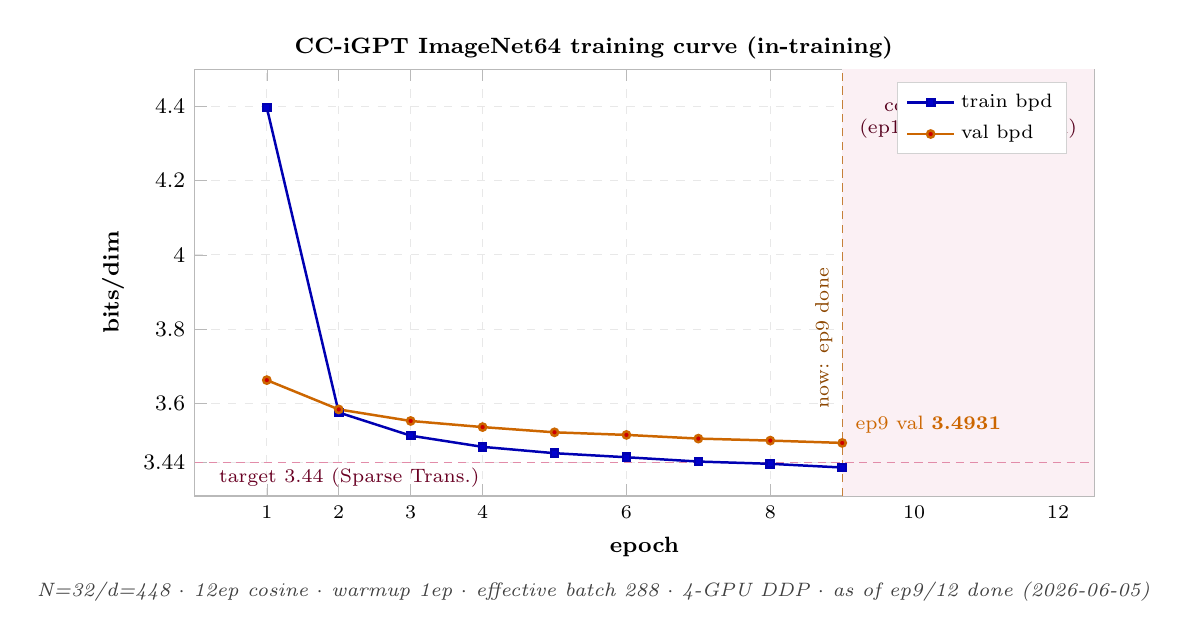
\begin{tikzpicture}[font=\footnotesize]
\begin{axis}[
    width=13cm, height=7cm,
    xlabel={\textbf{epoch}},
    ylabel={\textbf{bits/dim}},
    ylabel near ticks,
    xlabel near ticks,
    xmin=0, xmax=12.5,
    ymin=3.35, ymax=4.5,
    ytick={3.44,3.6,3.8,4.0,4.2,4.4},
    xtick={1,2,3,4,6,8,10,12},
    x tick label style={font=\scriptsize},
    axis line style={gray!55},
    tick style={gray!55},
    grid=major,
    grid style={dashed, gray!18, line width=0.3pt},
    legend style={
        font=\scriptsize,
        draw=gray!35, fill=white,
        at={(0.97,0.97)}, anchor=north east,
        cells={anchor=west},
        row sep=1pt,
    },
    clip=false,
]

% --- 退火尾段区间底纹 (ep10-12，待回填) ---
\fill[purple!6] (axis cs:9,3.35) rectangle (axis cs:12.5,4.5);
\node[font=\scriptsize, purple!45!black, anchor=north, align=center]
    at (axis cs:10.75, 4.45) {cosine anneal tail\\(ep10--12, not yet run)};

% --- 当前进度竖虚线 (ep9 done) ---
\draw[densely dashed, gray!45!orange, line width=0.4pt]
    (axis cs:9, 3.35) -- (axis cs:9, 4.5);
\node[font=\scriptsize, orange!55!black, anchor=south west, rotate=90]
    at (axis cs:9, 3.55) {\,now: ep9 done};

% --- 目标线 3.44 (Sparse Transformer) ---
\draw[densely dashed, purple!45, line width=0.5pt]
    (axis cs:0,3.44) -- (axis cs:12.5,3.44);
\node[font=\scriptsize, purple!55!black, anchor=west]
    at (axis cs:0.2, 3.40) {target 3.44 (Sparse Trans.)};

% --- train_bpd 曲线 (9 点) ---
\addplot+[
    mark=square*, mark size=1.3pt, line width=0.9pt, color=blue!70!black,
] coordinates {
    (1, 4.3969)
    (2, 3.5751)
    (3, 3.5127)
    (4, 3.4825)
    (5, 3.4654)
    (6, 3.4545)
    (7, 3.4429)
    (8, 3.4368)
    (9, 3.4268)
};
\addlegendentry{train bpd}

% --- val_bpd 曲线 (9 点) ---
\addplot+[
    mark=*, mark size=1.3pt, line width=0.9pt, color=orange!80!black,
] coordinates {
    (1, 3.6624)
    (2, 3.5834)
    (3, 3.5523)
    (4, 3.5358)
    (5, 3.5217)
    (6, 3.5147)
    (7, 3.5048)
    (8, 3.4994)
    (9, 3.4931)
};
\addlegendentry{val bpd}

% --- ep9 末点标注 ---
\node[font=\scriptsize, orange!80!black, anchor=south west]
    at (axis cs:9.05, 3.4931) {ep9 val \textbf{3.4931}};

\end{axis}

% --- 标题 ---
\node[font=\footnotesize\bfseries, anchor=south]
    at (current bounding box.north)
    {CC-iGPT ImageNet64 training curve (in-training)};

% --- 副标题（配置） ---
\node[font=\scriptsize, gray!50!black, anchor=north, yshift=-2pt]
    at (current bounding box.south)
    {\textit{N=32/d=448 $\cdot$ 12ep cosine $\cdot$ warmup 1ep $\cdot$ effective batch 288 $\cdot$ 4-GPU DDP $\cdot$ as of ep9/12 done (2026-06-05)}};

\end{tikzpicture}
\end{document}
